\documentclass[a6paper, 12pt, parskip=half, DIV=14]{scrartcl}

\usepackage[dvipsnames]{xcolor}
\usepackage{tikz}
\usepackage{subcaption}
\usepackage{float}
\usepackage{ragged2e}
% Minimize unwanted hyphenation
\tolerance=1
\emergencystretch=\maxdimen
\hyphenpenalty=1
\hbadness=10000

\usepackage{fontspec}
\setmainfont{Tex Gyre Schola}
%\setmainfont{Qwigley}

\usepackage{eso-pic}
\usepackage{contour}
\contourlength{0.25mm}
\contournumber{1024}

\definecolor{SunriseBlue}{HTML}{0482ba}
%\definecolor{SunriseBlue}{HTML}{A9C2E5}
\setkomafont{section}{\setmainfont{Quicksand-Bold}\LARGE\color{SunriseBlue}}
\setkomafont{subsection}{\setmainfont{Quicksand-Bold}\Large\color{SunriseBlue}}
\setkomafont{subsubsection}{\setmainfont{Quicksand-Bold}\large\color{SunriseBlue}}

% Adjust spacing before and after section headings
\RedeclareSectionCommand[
  runin=false,
  beforeskip=0.5\baselineskip,
  afterskip=-0.0\baselineskip
]{section}

% Adjust spacing before and after subsection headings
\RedeclareSectionCommand[
  runin=false,
  beforeskip=0.5\baselineskip,
  afterskip=-0.0\baselineskip
]{subsection}

% Adjust spacing before and after subsubsection headings
\RedeclareSectionCommand[
  runin=false,
  beforeskip=0.5\baselineskip,
  afterskip=-0.0\baselineskip
]{subsubsection}


\usepackage{enumitem}
\setlist[description]{labelindent=0pt, labelsep=\widthof{ }, leftmargin=\widthof{\textbf{License: }}, font=\setmainfont{Tex Gyre Schola}\bfseries}

\usepackage[hang,flushmargin]{footmisc}
\newcommand\blfootnote[1]{%
  \begingroup
  \renewcommand\thefootnote{}\footnote{#1}%
  \addtocounter{footnote}{-1}%
  \endgroup
}

\renewcommand{\thefootnote}{\fnsymbol{footnote}}
\renewcommand{\footnoterule}{%
  \kern -3pt
  \hrule width \textwidth height 0.5pt
  \kern 2pt
}

\usepackage[hidelinks]{hyperref}
\usepackage[type={CC}, version={4.0}, modifier={by-sa}]{doclicense} % Add text and icons for creative commons license
%\usepackage{array}

\raggedright
\pagestyle{empty}
%\pagecolor{SkyBlue!50}
\begin{document}

\begin{titlepage}
\AddToShipoutPictureBG{
\begin{tikzpicture}[remember picture, overlay]
%	\node () at (current page.center) {\includegraphics[width=\pagewidth, height=\pageheight]{Images/aloft_cover_background.png}};
	\node () at (current page.center) {
\includegraphics[width=\pagewidth, height=\pageheight]{Images/skyfire_front_cover.png}};
\end{tikzpicture}
}
\phantom{SkyFire}
\end{titlepage}


\ClearShipoutPicture
\enlargethispage{1.75\baselineskip}
\section*{Overview}
SkyFire is a game of wits, deception, and social deduction for three to five players. It can be played in about thirty minutes and is intended for players who are at least twelve years old.

During the game, you will work with your opponents to build collections of fireworks. A complete game plays out over a series of five rounds.

Each round, you will given a target. To score points, you will need to be the first player to correctly guess when one of those collections satisfies that target. The player with the most points after five rounds wins the game.

\newpage
\enlargethispage{1.75\baselineskip}
\section*{Components}
    \begin{itemize}[nosep, leftmargin=*]
      \item 20 fireworks cards 
      	\vspace{-1ex}      
			\begin{figure}[H]
			\centering
				\begin{subfigure}{0.3\textwidth}
				\centering
					
\includegraphics[width=0.66\textwidth]{Images/fireworks_card_back_display.png}
					\caption*{{\scriptsize Back}}
				\end{subfigure}
				\begin{subfigure}{0.3\textwidth}
				\centering
				 
\includegraphics[width=0.66\textwidth]{Images/fireworks_card_front_display.png} 
				 \caption*{{\scriptsize Front}}
				 \end{subfigure} 
			\end{figure}      
%	\vspace{-2ex}      
      \item 10 target cards
      	\vspace{-1ex}      
			\begin{figure}[H]
			\centering
				\begin{subfigure}{0.3\textwidth}
				\centering
					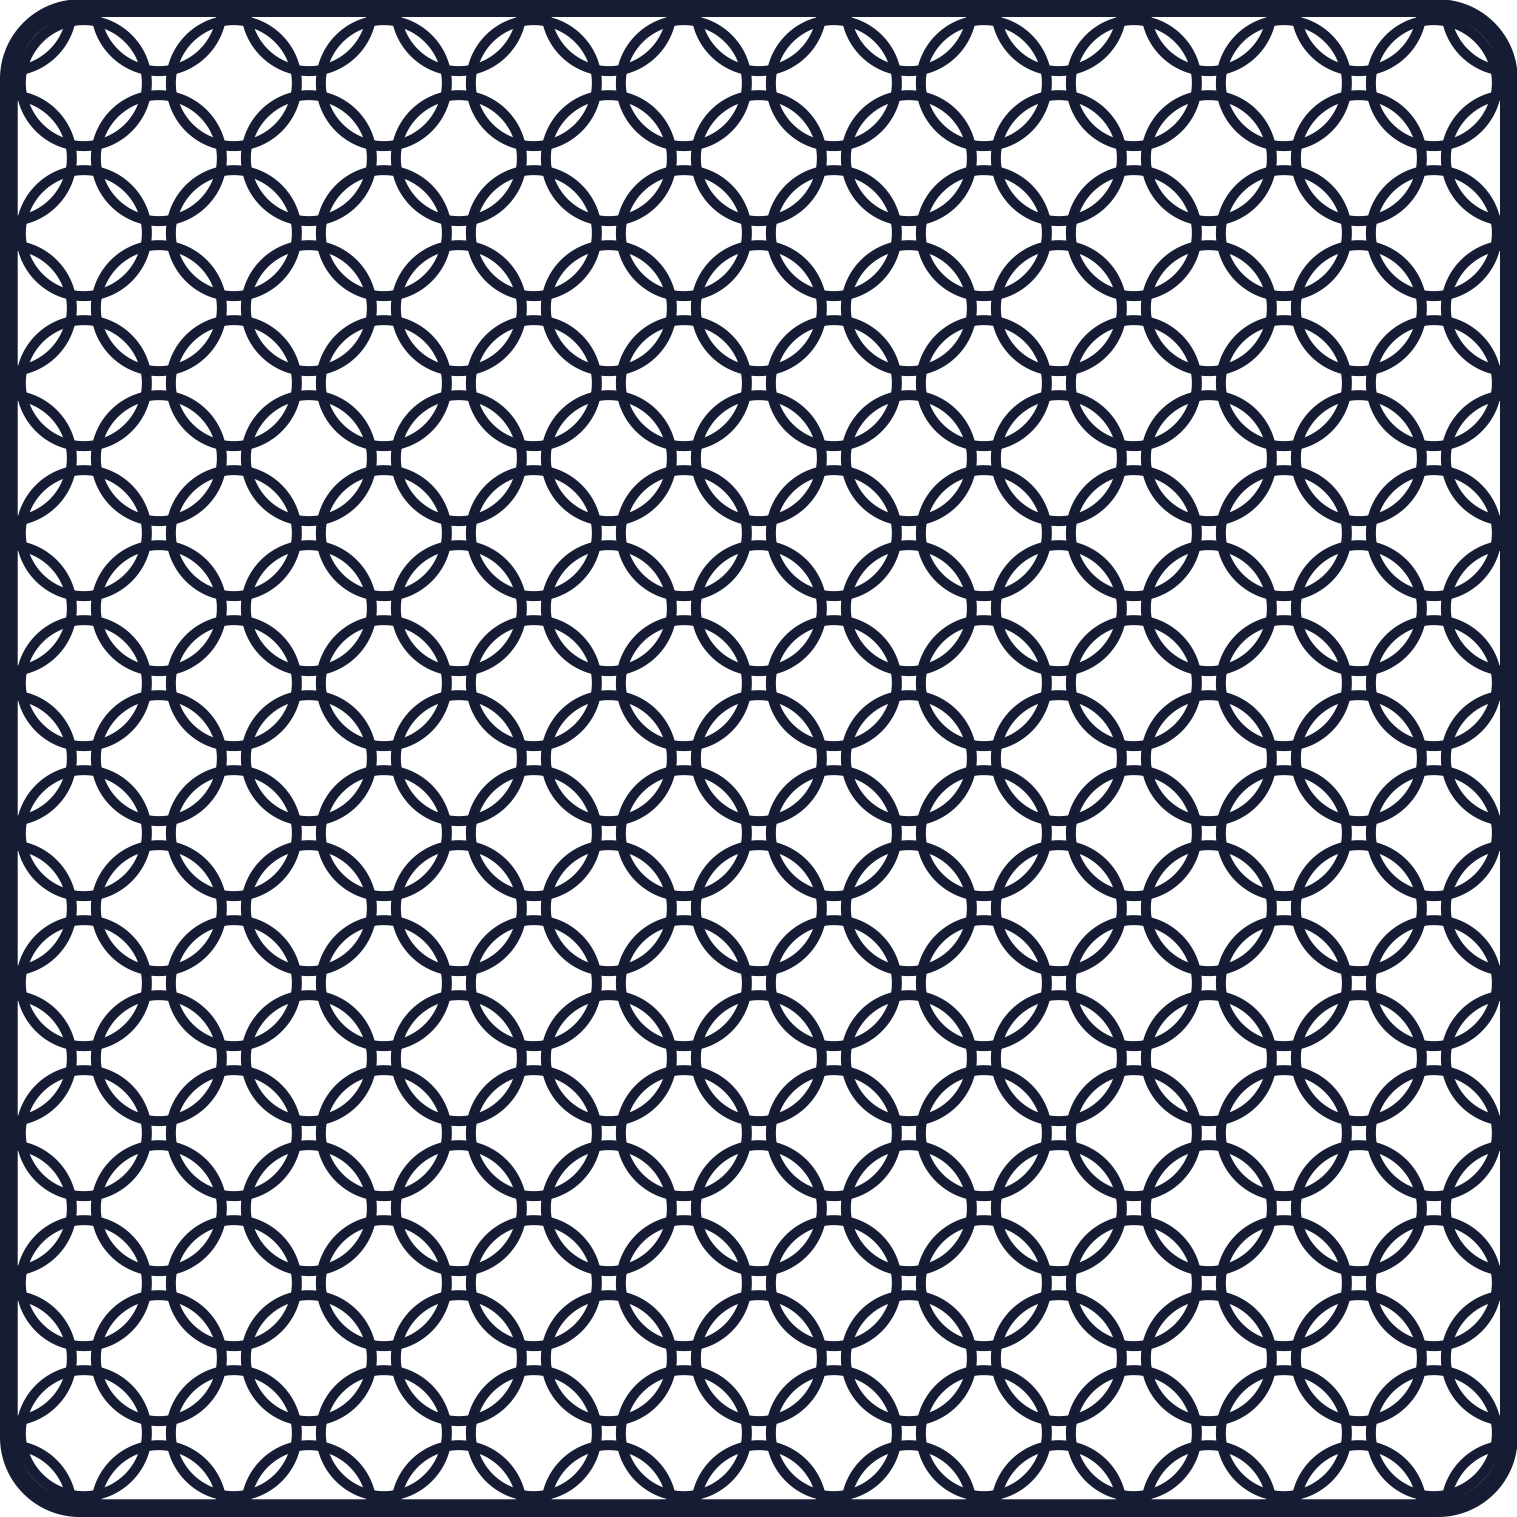
\includegraphics[width=0.66\textwidth]{Images/target_card_back_display.png}
					\caption*{{\scriptsize Back}}
				\end{subfigure}
				\begin{subfigure}{0.3\textwidth}
				\centering
				 
\includegraphics[width=0.66\textwidth]{Images/target_card_front_display.png} 
				 \caption*{{\scriptsize Front}}
				 \end{subfigure} 
			\end{figure}      
%	\vspace{-2ex}      
      \item 2 finale cards
      	\vspace{-1ex}      
			\begin{figure}[H]
			\centering
				\begin{subfigure}{0.3\textwidth}
				\centering
					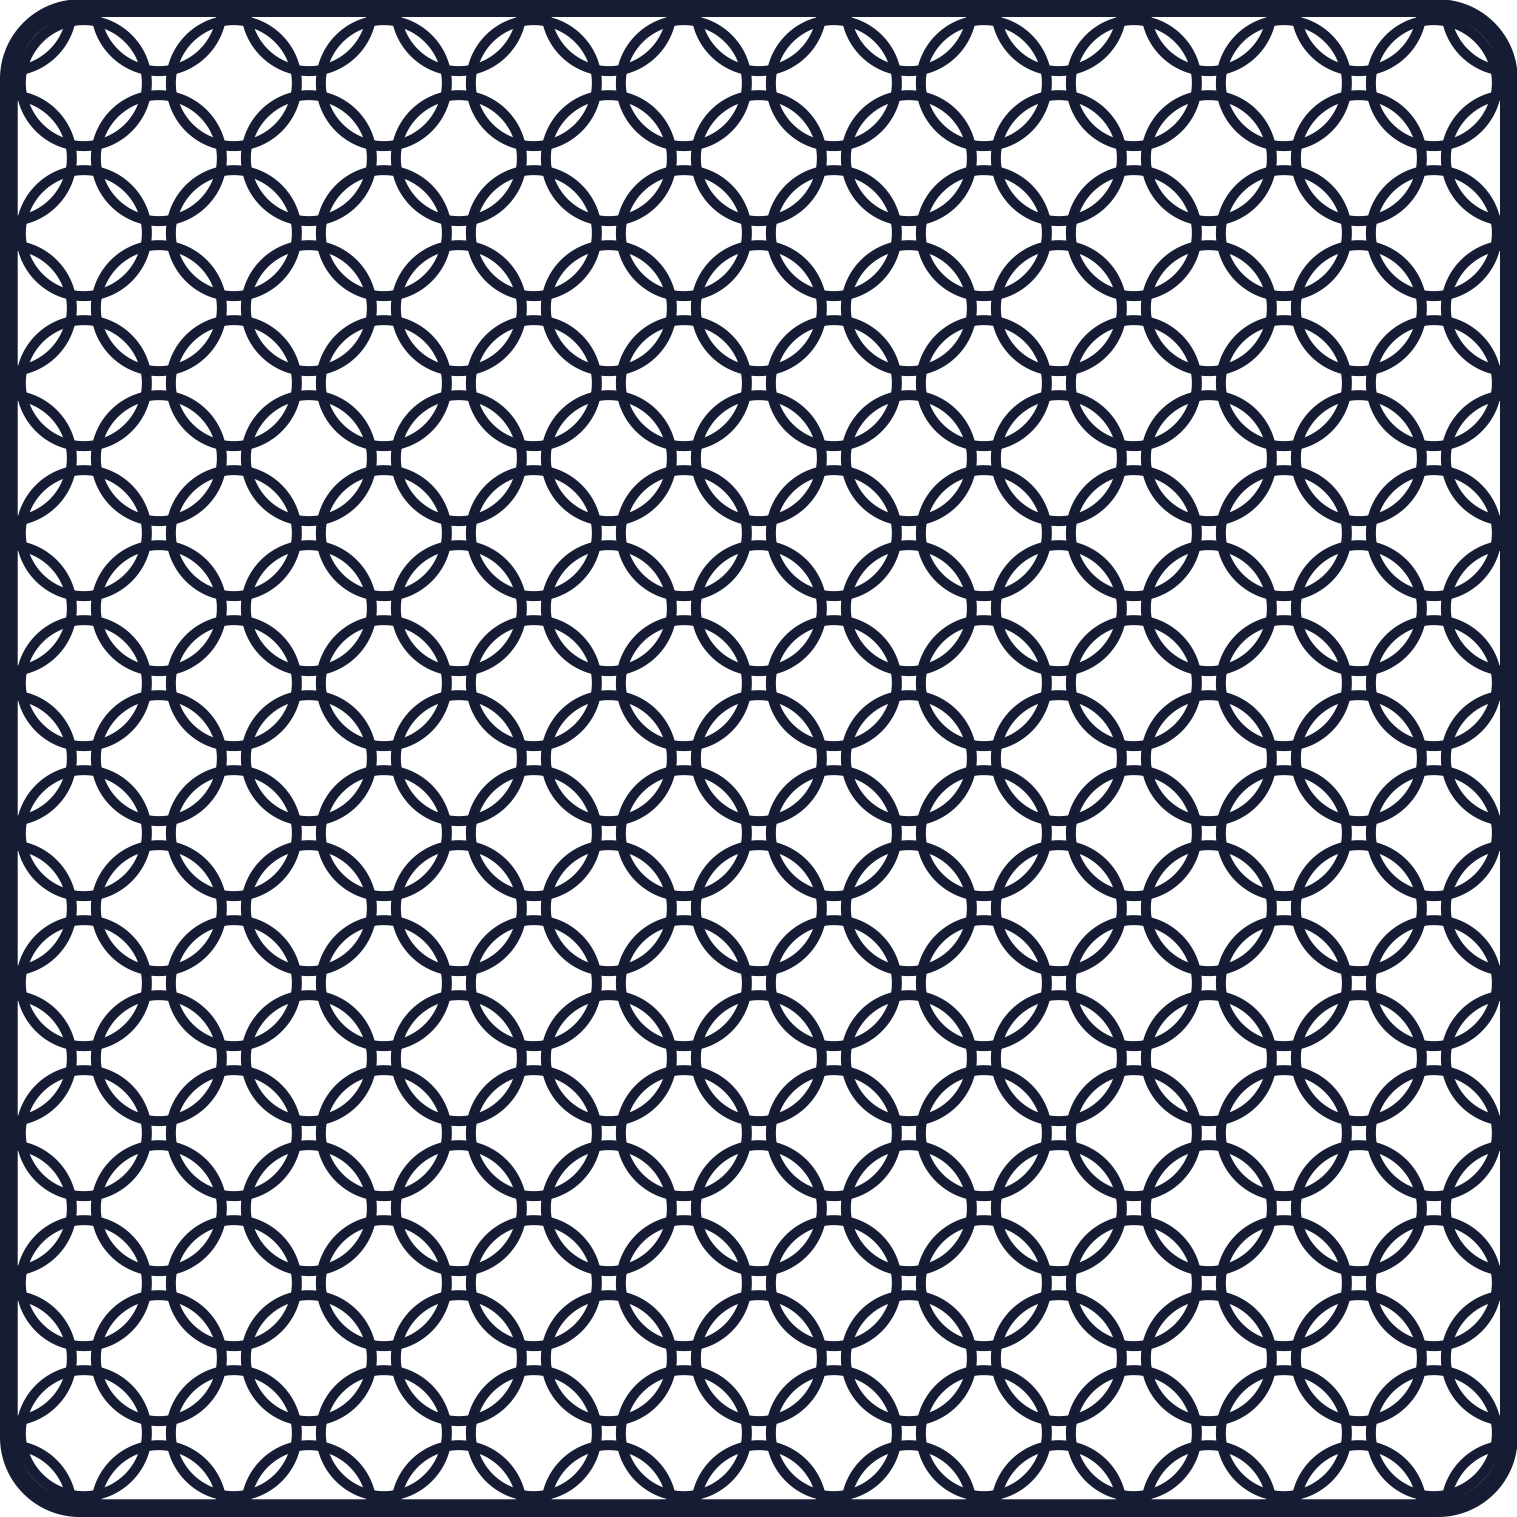
\includegraphics[width=0.66\textwidth]{Images/target_card_back_display.png}
					\caption*{{\scriptsize Back}}
				\end{subfigure}
				\begin{subfigure}{0.3\textwidth}
				\centering
					
\includegraphics[width=0.66\textwidth]{Images/finale_card_4_display.png}
					\caption*{{\scriptsize Front (3 Players)}}
				\end{subfigure}
				\begin{subfigure}{0.3\textwidth}
				\centering
				 
\includegraphics[width=0.66\textwidth]{Images/finale_card_5_display.png} 
				 \caption*{{\scriptsize Front (4/5 Players)}}
				 \end{subfigure}
			\end{figure}      
    \end{itemize}

\newpage
\enlargethispage{1.75\baselineskip}
\section*{Prepare the Decks}
You will use different numbers of the various types of cards depending on how many players you have.

  \begin{description}[leftmargin=0pt]
    \item[Three Players:] Remove every card that displays any white fireworks symbols. Set aside two of the target cards that you removed to use as launch-zone cards.

    \item[Four Players:] Remove any six target cards and the three-player finale card. Set aside three of the target cards that you removed to use as launch-zone cards.
    
    \item[Five Players:] Remove any six target cards and the three-player finale card. Set aside four of the target cards that you removed to use as launch-zone cards.
  \end{description}

\newpage
\enlargethispage{1.75\baselineskip}
\section*{Game Set Up}
Before the start of the game, you will do the following:
\begin{enumerate}[leftmargin=*]
  \item Place the finale card face up in the middle of the play area.

  \item Shuffle the target cards.
    
  \item Place the target cards face up in a single stack on top of the finale card.
  
  \item Place the launch-zone cards face down in the play area. Ensure that no two launch-zone cards are placed close to one another.

\end{enumerate}

\newpage
\enlargethispage{1.75\baselineskip}
\section*{Round Set Up}
Before the start of each round, you will do the following:
\begin{enumerate}[leftmargin=*]
  \item Shuffle the fireworks cards.
  
  \item Deal four fireworks cards face down to each player.
  
  \item For a four-player game, you will have four fireworks cards left over. Display these cards face down near the play area with their backs clearly visible.
  
  \item Identify the target. The target is the set of fireworks symbols displayed on the topmost card on the stack of target/finale cards.

\end{enumerate}

\newpage
\enlargethispage{1.75\baselineskip}

\section*{Gameplay}
On your turn, you will perform a single action. You will either place fireworks, launch fireworks, or declare a misfire.

After you launch fireworks or declare a misfire, you will check to see if one or more collections of fireworks satisfies the target for the current round. A collection satisfies a target if every fireworks symbol that in the target set appears on the faces of the cards in that collection.

\subsection*{Place Fireworks}
To place fireworks, you will add one fireworks card from your hand to one of the launch zones. Place your fireworks card face down with its back clearly visible near one of the launch-zone cards.  

If you do not have any fireworks cards in your hand at the start of your turn, you cannot place fireworks. You must either launch fireworks or declare a misfire.
\newpage
\enlargethispage{1.75\baselineskip}
\subsection*{Launch Fireworks}
To launch fireworks, you will reveal all of the cards in any one of the launch zones so that they are face up.

If the collection of fireworks that you launched satisfy the target, then you win the round and will score points. If not, then you are eliminated from the round.

\subsection*{Declare a Misfire}
If you do not have any fireworks cards remaining in your hand at the start of your turn, then you may declare a misfire. To do so, reveal all of the cards in every launch zone so that they are face up.

Check to see if the any of the collections of fireworks satisfy the target. If not, then you win the round and you will score points. Otherwise, all players who have not been eliminated win the round and will score points.

\newpage
\enlargethispage{1.75\baselineskip}
\subsection*{Scoring}
You will score points every time that you win a round.
\blfootnote{\textbf{Design}: Michael Purcell}
\blfootnote{\textbf{Contact}: \href{mailto:skyfire.card.game@gmail.com}{skyfire.card.game@gmail.com}}
\blfootnote{\textbf{License}: \raggedright\doclicenseText}

If you win a round by launching a collection of fireworks that satisfies the target, you score one point for every fireworks card in that collection.

If you win a round by correctly declaring a misfire, you score one point for each card in the largest collection you revealed.

If you win a round by having one of your opponents incorrectly declare a misfire, you score three points. 
 \newpage
 \AddToShipoutPictureBG{
\begin{tikzpicture}[remember picture, overlay]
	\node () at (current page.center) {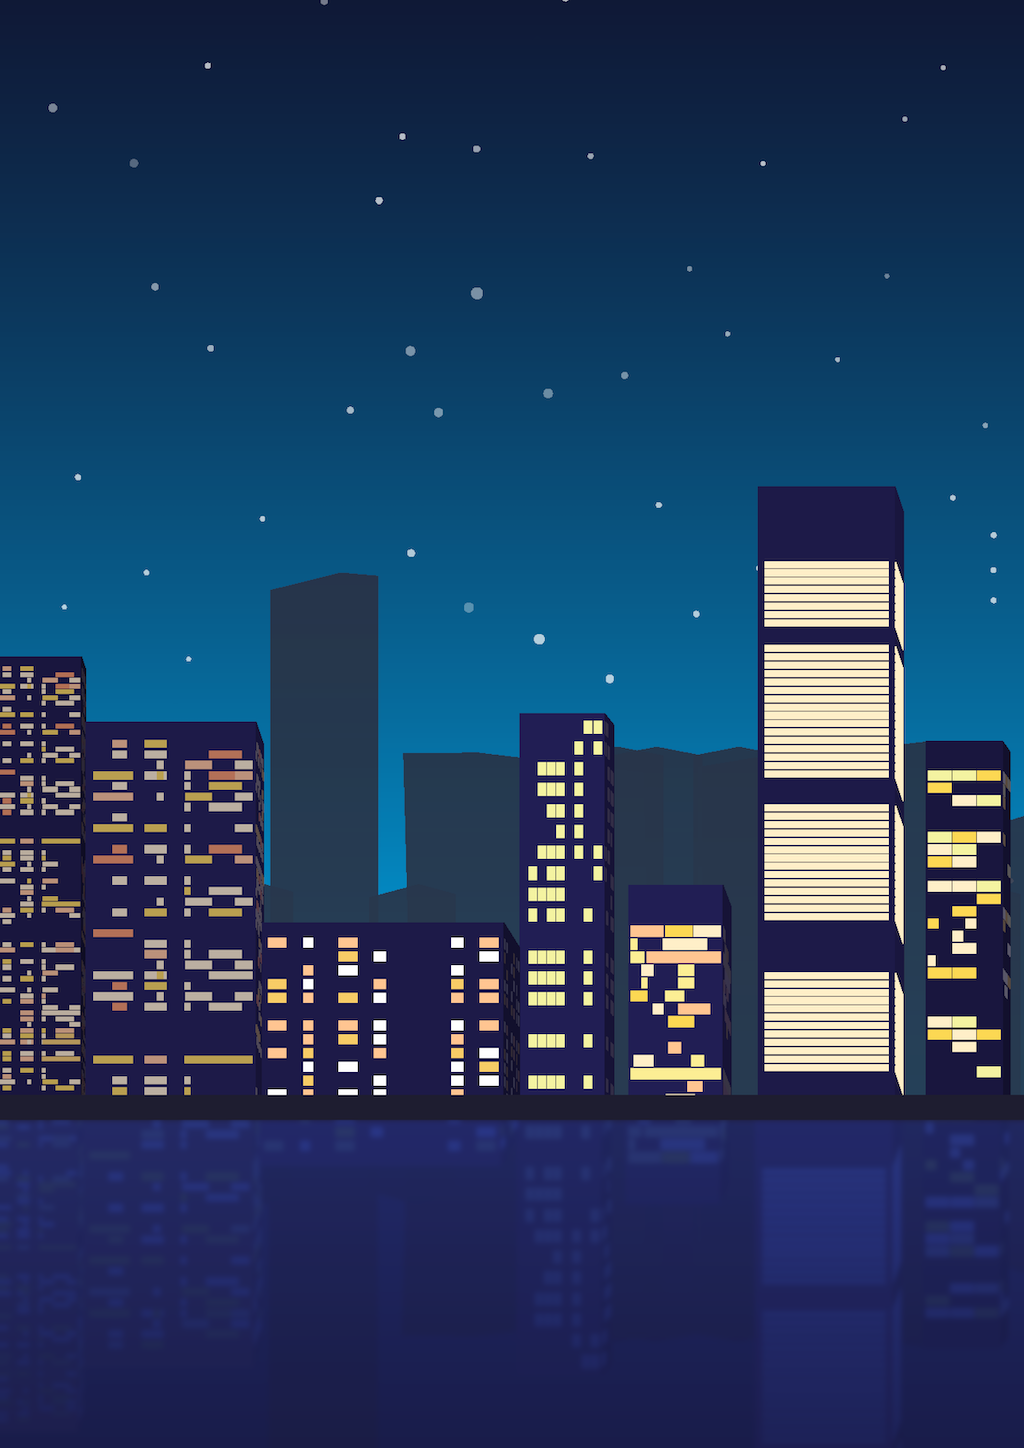
\includegraphics[width=\pagewidth, height=\pageheight]{Images/skyfire_back_cover.png}};
\end{tikzpicture}
}
\phantom{SkyFire}
\end{document}